\documentclass{article}
\usepackage{graphicx}
\begin{document}
Tameez Latib

Problem 8

I, Tameez Latib, declare that this work is my own. I did this work honestly and can fully stand behind everything that I have written.

---

One model for foxes and rabbits could be that the rabbits increase with a rate $\alpha$, (the combined birth - death rate of rabbits) but decrease when they're eaten by foxes. The amount of rabbits eaten should be proportional to the foxes (more foxes, obviously more rabbits are eaten) and also the rabbits (the more rabbits, the more food for the foxes so they don't have to conserve their food). Let's call the proportionality constant n. Therefore,

$R' = \alpha R - n RF$

The amount of foxes similarly increases with a rate $\gamma$, (the combined birth - death rate of foxes). However, it decreases if the foxes starve. So we need to take into account that the number of new members joining the fox group should depend on how many foxes are starving. The number of foxes starving should be proportional to foxes, as more foxes implies less food, and inversely proportional to rabbits, as more rabbits implies more food. Let's call the proportionality constant $\lambda$. So,

$F' = \gamma F - \gamma F (\lambda \frac{F}{R}) =  \gamma F(1 - (\lambda \frac{F}{R}))$

By dimensional analysis: 

$F = f*\bar{f}$

$R = r*\bar{r}$

$t = \tau \bar{t}$

and thus

$$\frac{dF}{dt} = \frac{df}{d\tau}*{\bar{f}}/{\bar{t}}$$

$$\frac{dR}{dt} = \frac{dr}{d\tau}*{\bar{r}}/{\bar{t}}$$

Substituting in the new variables,

$$ \frac{dr}{d\tau}*{\bar{r}}/{\bar{t}} = \alpha r\bar{r} - n \bar{r}\bar{f}rf$$

$$ \frac{dr}{d\tau} = \alpha r\bar{t} - n \bar{t}\bar{f}rf$$

Let $\bar{t} = 1/\alpha$, $\bar{f} = \alpha/n$

$$\frac{df}{d\tau}*{\bar{f}}/{\bar{t}}  = \gamma f*\bar{f}(1 - (\lambda \frac{f*\bar{f}}{r*\bar{r}}))$$

$$\frac{df}{d\tau}  = \gamma f*\bar{t}(1 - (\lambda \frac{f*\bar{f}}{r*\bar{r}}))$$

Let $\gamma*\bar{t} = \sigma$, a variable based on $\gamma$, and  $\bar{r} = \lambda*\alpha/n$

Now our equations simplify to 

$$ \frac{dr}{d\tau} = r - rf = r(1 - f)$$

$$\frac{df}{d\tau}  = \sigma f(1 - \frac{f}{r})$$

let's use a numeric method (Euler's method) to graph r and f, with initial value $r(0) = 1$, $f(0) = 1$


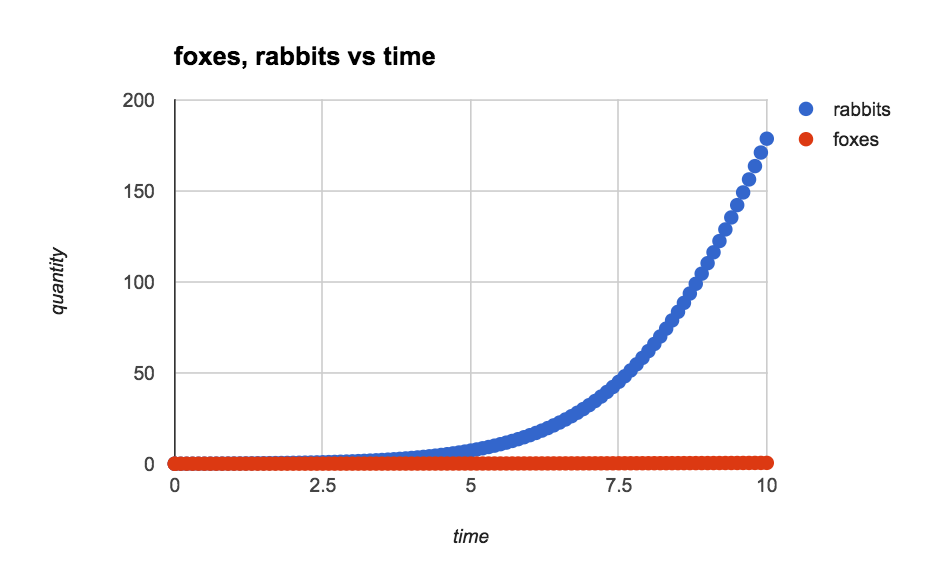
\includegraphics[width=10cm, height=7cm]{2RabFox}

\textbf{Figure 1} Graph of rabbits and foxes vs time for $\sigma = 0.2$ 
\vspace{1cm}

This makes sense as for low values of $\sigma$, $\gamma$ is low, meaning that the influx of foxes is very low. As seen in the graph, the fox population is increasing ever so slightly, yet on the scale of the increase in the population of the rabbits, it seems like almost nothing. The rabbits seem to increase without bound, and this makes sense as there are virtually no foxes compared to the huge amount of rabbits. Also, intuitively, rabbits breed extremely fast, and without and killers (foxes), their population skyrockets. However, eventually the fox population will increase to a point such that they can eat a lot of rabbits, 

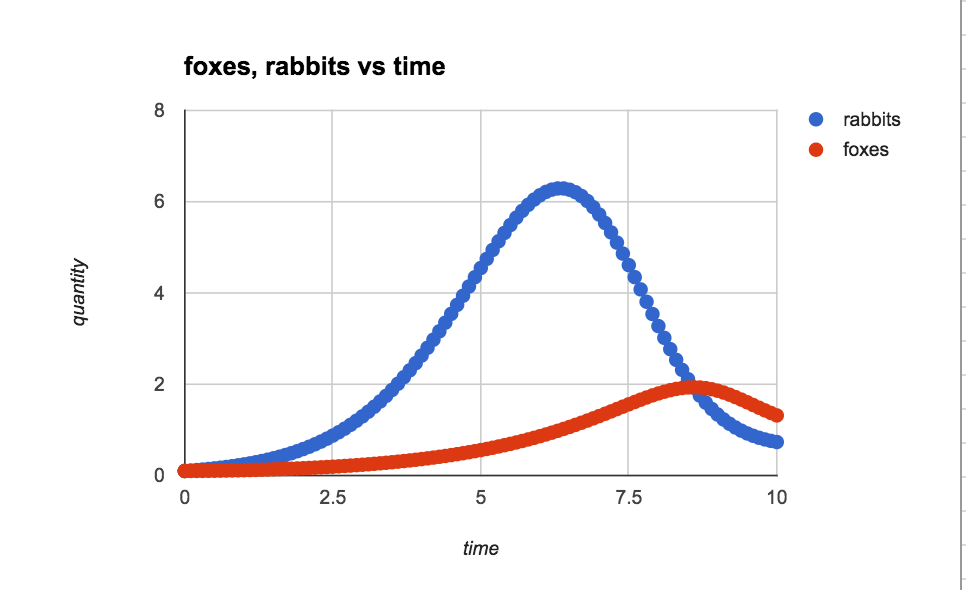
\includegraphics[width=10cm, height=7cm]{5RabFox}

\textbf{Figure 1} Graph of rabbits and foxes vs time for $\sigma = 0.5$ 
\vspace{1cm}

Here, $\gamma$ is much higher and so the amount of new foxes entering the population is higher. As seen from the graph, the foxes increase slowly at first, because there aren't that many of them. The rabbits, on the other hand, increase extremely rapidly (rabbits breed really fast). However, as the fox population increases, the number of rabbits starts to decline as they eat more than the rabbits reproduce. As the rabbit population goes down, the fox population eventually goes down because there aren't enough rabbits. In fact, a higher $\sigma$ value simply expedites the process, that is, as $\sigma$ increases, the time it takes for the cycle (rabbits increase so foxes increase so rabbits decrease so foxes decrease and repeat) goes down.


\end{document}
